\documentclass[12pt,letterpaper]{article}
\usepackage[utf8]{inputenc}
\usepackage{listings, float, xcolor}

%----- Configuración del estilo del documento------%
\usepackage{graphicx, fancyhdr}
\usepackage{enumitem, pifont, hyperref, ulem, tabularx}
\usepackage[left=2cm,right=2cm,top=1.8cm,bottom=2.3cm]{geometry}
\usepackage{hyperref}
\usepackage{lastpage}


%------ Paquetes matemáticos básicos --------%
\usepackage{amsmath, amssymb, amsthm}

%------ Definimos los colores para la sintaxis del código --------%
\definecolor{keywordcolor}{rgb}{0.5, 0.0, 0.5}  % Morado para palabras clave
\definecolor{commentcolor}{rgb}{0.25, 0.5, 0.35} % Verde para comentarios
\definecolor{stringcolor}{rgb}{0.88, 0.68, 0.18}  % Mostaza anaranjado para los strings
\definecolor{backgroundcolor}{rgb}{0.95, 0.95, 0.95} % Gris claro para fondo

%------ Configuración para mostrar código en C++ --------%
\lstdefinestyle{cppstyle}{
    language=C++,
    basicstyle=\ttfamily\footnotesize,
    keywordstyle=\color{keywordcolor}\bfseries,
    commentstyle=\color{commentcolor},
    stringstyle=\color{stringcolor},
    numbers=left,
    numberstyle=\tiny,
    stepnumber=1,
    numbersep=8pt,
    backgroundcolor=\color{backgroundcolor},
    tabsize=2,
    showspaces=false,
    showstringspaces=false,
    breaklines=true,
    frame=single,
    captionpos=b
}

%------ Configuración para mostrar código en MIPS --------%
\lstdefinelanguage{MIPS}{
  morekeywords={li, la, syscall, add, sub, mul, div, l, s}, 
  sensitive=true,
  morecomment=[l]{#},  % Comentarios con #
  morestring=[b]",     % Strings entre comillas
}

\lstdefinestyle{mipsstyle}{
    language=MIPS,
    basicstyle=\ttfamily\footnotesize,
    keywordstyle=\color{keywordcolor}\bfseries,
    commentstyle=\color{commentcolor},
    stringstyle=\color{stringcolor},
    numbers=left,
    numberstyle=\tiny,
    stepnumber=1,
    numbersep=8pt,
    backgroundcolor=\color{backgroundcolor},
    tabsize=2,
    showspaces=false,
    showstringspaces=false,
    breaklines=true,
    frame=single,
    captionpos=b,
    morekeywords={.data, .text, .globl, l.d, add.d, add.s} % Agregar palabras clave especiales aquí
}


\hypersetup{
    colorlinks=true,
    linkcolor=blue!50!black, % Azul oscuro
    urlcolor=blue!50!black,  % Azul oscuro
    hidelinks % Elimina el recuadro azul
}

\begin{document}

%------ Encabezado -------- %
\begin{center}
  \begin{minipage}{3cm}
    \begin{center}
      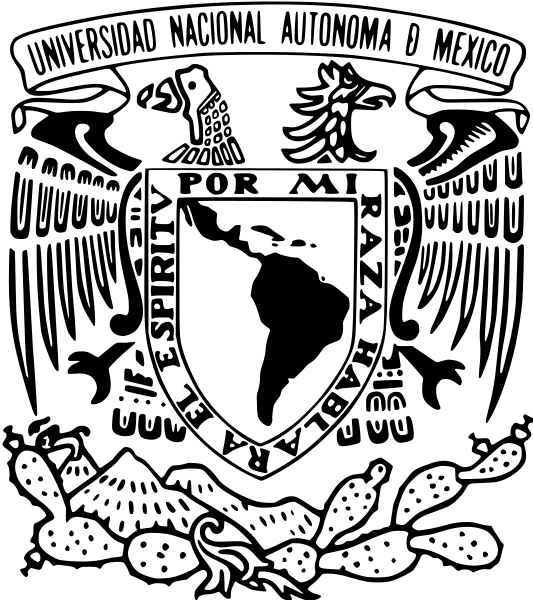
\includegraphics[height=3.4cm]{../unam_logo.png}
    \end{center}
  \end{minipage}\hfill
  \begin{minipage}{10cm}
    \begin{center}
      \textbf{\Large Universidad Nacional Autónoma de México}\\[0.2cm]
      \textbf{\large Facultad de Ciencias}\\[0.2cm]
      \textbf{Organización y Arquitectura de Computadoras 2025-2}\\[0.4cm]
      \textbf{\Large Práctica 07}\\[0.1cm]
      \textbf{Docentes:}\\
      José Galaviz \hspace{1em} Ricardo Pérez \hspace{1em} Ximena Lezama\\[0.3cm]
      \textbf{Autores:}\\
      Fernanda Ramírez Juárez \quad Ianluck Rojo Peña\\[0.3cm]
      \textbf{Fecha de entrega:} Jueves 3 de abril de 2025
    \end{center}
  \end{minipage}\hfill
  \begin{minipage}{3cm}
    \begin{center}
      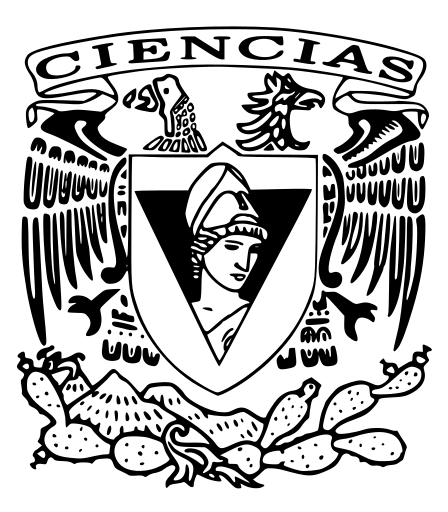
\includegraphics[height=3.4cm]{../fc_logo.png}
    \end{center}
  \end{minipage}
\end{center}

\bigskip
\hrule height 0.1pt
\bigskip

%------ Contenido -------- %
\section*{Ejercicios.}

\subsection*{Ejercicio 1.}

\begin{lstlisting}[style=cppstyle, caption={Código en C++ ~ Calculador de Serie}]
#include <iostream>
using namespace std;

//Funcion que implementa la serie de Leibniz con el que nos aproximamos al valor de pi
int main() {
  cout << "Ingrese un valor para m: ";
  int m;          //Creamos la varible m para los terminos de la serie
  cin >> m;       //Leemos la varible del usuario
  float r = 0.0f; //El resultado a imprimir
  
  //Bucle para realizar la serie hasta los m terminos
  for (int n = 0; n <= m; n++) {
    //Calculamos cada termino de la serie, alternamos los valores de 1 y -1
    float j = ((n % 2 == 0) ? 1.0f : -1.0f) / ((2.0f * n) + 1.0f);
    r += j; //Sumamos la division obtenida a nuestros resultados previos 
  }
  
  cout << "Resultado de la serie: " << r * 4.0f << endl;
}
\end{lstlisting}

\newpage

\subsection*{Ejercicio 4.}

Razones por las cuales se asignaron los siguientes valores a las variables utilizadas en el cálculo:

\textbf{Constante de gravitación universal (G)}
 
\begin{itemize}
\item Valor asignado: $6.674e-11 = 6.67430 \times 10^{-11}$.
  
\item Este valor, adem\'{a} de ser tomado como referencia en el archivo pdf para la pr\'{a}ctica 7; es una constante física obtenida de forma empírica, que determina la intensidad de la fuerza de atracción gravitatoria entre los cuerpos. Se denota por $G$ y aparece tanto en la ley de gravitación universal de Newton como en la teoría general de la relatividad de Einstein. La medida de G fue obtenida implícitamente por primera vez por Henry Cavendish en 1798. El valor actual corresponde al valor oficial publicado por CODATA de la forma:
  
  \begin{center}
  $6.67430 \times 10^{-11} \frac{N \cdot m^2}{kg^2}$
  \end{center}

\item Fuente: \href{https://es.wikipedia.org/wiki/Constante_de_gravitaci\%C3\%B3n_universal}{Wikipedia - Constante de gravitación universal}.
\end{itemize}


\textbf{Masa de la Tierra:}

\begin{itemize}
\item Valor asignado: $5.9722e24 = 5.9722 \times 10^{24}$.
  
\item Este valor es ampliamente aceptado y corresponde a la mejor estimación actual con una incertidumbre relativa de $10^{-4}$.
  
\item Fuente: \href{https://en.wikipedia.org/wiki/Earth_mass}{Wikipedia - Earth Mass}.
\end{itemize}

\textbf{Masa de la Luna:}

\begin{itemize}
\item Valor asignado: $7.349e22 = 7.349 \times 10^{22}$.
  
\item Valor aceptado en astronomía y utilizado en cálculos de fuerza gravitacional.
  
\item Fuente: \href{https://es.wikipedia.org/wiki/Luna}{Wikipedia - Luna}.
\end{itemize}

\textbf{Distancia entre la Tierra y la Luna:}

\begin{itemize}
\item Valor asignado: $384400.0$.
  
\item Basado en la información proporcionada por la NASA.
  
\item Fuente: \href{https://spaceplace.nasa.gov/moon-distance/sp/}{NASA Space Place}.
\end{itemize}

\textbf{Cálculo de la Fuerza Gravitacional:}

Como se puede observar, en el programa en ensamblador para el ejercicio 4, el resultado obtenido es:

\begin{equation}
  1.9823577584943926E26 = 1.9823577584943926 \times 10^{26}
\end{equation}

Tomando como referencia el trabajdo realizado porFernández, J. L. en: \href{https://www.fisicalab.com/ejercicio/898}{Fisicalab - Fuerza de la Luna}

El cual toma valores muy aproximados a los utilizados para el programa en ensamblador:\\

Masa de la Tierra $= M_T = 5.98 \times 10^{24} kg$

Masa de la Lunea $= M_L = 7.34 \times 10^{22} kg$

Distancia de la Tierra a la Luna $= R = 384 \times 10^3 km = 384 \times 10^6 m$

Fuerza Gravitacional = G $= 6.67430 \times 10^{-11} \frac{N \cdot m^2}{kg^2}$

Aplicando la ley de gravitación universal:

\begin{equation}
    F = G \cdot \frac{M_T \cdot M_L}{R^2}
\end{equation}

Sustituyendo los valores:

\begin{equation}
    F = 6.674 \times 10^{-11} \cdot \frac{(5.9722 \times 10^{24}) \cdot (7.349 \times 10^{22})}{(3.844 \times 10^{8})^2} = 1.98 \times 10^{20}
\end{equation}

Notemos que el resultado es similar, dentro del margen esperado debido a las diferencias en las cifras significativas y redondeos.

\subsection*{Referencias.}

\begin{itemize}
\item Colaboradores de Wikipedia. \textbf{(2025, enero 29)}. \textit{Constante de gravitación universal}. [Wikipedia, la Enciclopedia Libre]. \url{https://es.wikipedia.org/wiki/Constante_de_gravitaci%C3%B3n_universal}
  
\item Contributors to Wikimedia projects. \textbf{(2025, 28 marzo)}. \textit{Earth mass}. [Wikipedia, la Enciclopedia Libre].. \url{https://en.wikipedia.org/wiki/Earth_mass}
  
\item Colaboradores de Wikipedia. \textbf{(2025, marzo 26}). \textit{Luna}. [Wikipedia, la Enciclopedia Libre].. \url{https://es.wikipedia.org/wiki/Luna}
  
\item NASA. \textbf{(s. f.}). \textit{How Far Away Is the Moon?}. [NASA]. \url{https://spaceplace.nasa.gov/moon-distance/sp/}
  
\item Fernández, J. L. \textbf{(s. f.}). \textit{Ejercicio: La fuerza de la Luna}. [Fisicalab]. \url{https://www.fisicalab.com/ejercicio/898}
  
\end{itemize}

\newpage

\section*{Preguntas.}

\begin{enumerate}
\item En el ejercicio 1:
  % -- Respuesta -- %
  \begin{itemize}
  \item ¿A qué valor tiende la serie?
    
    Cómo se mencionó en los comentarios del código, la serie es una serie de Leibniz la cual tiende al valor de pi $\pi$.

    Lo podemos comprobar fácilmente al ejecutar el código e ingresar valores relativamente grandes para m y esperar como salida 3.1416...\\
    
  \item ¿A cuántos dígitos estaría limitado nuestro resultado con precisión sencilla? (Flotante) Justifica tu respuesta.
    
    En C++ los valores para el tipo float maneja una precisión de entre 6 y 7 dígitos decimales.
    En ensamblador en MIPS los registro de punto flotante almacenan 32 bits, lo que nos da una precisión similar. Es decir la serie esta limitada con punto flotante de precisión sencilla a aproximadamente 6-7 dígitos significativos.\\
    
  \item ¿Cuántas iteraciones son necesarias para calcular el mayor número de dígitos?
    
    Cómo lo comentamos anteriormente, a medida que aumentamos el valor de m (el número de iteraciones en la serie de Leibniz) la aproximación a $\pi$ se vuelve más precisa.

    Sin embargo, debido a que el programa utiliza números de punto flotante, tenemos que el límite en la cantidad de dígitos exactos que podemos obtener es de 7; antes de que la precisión se vea afectada por los errores numéricos.

    Al ejecutar el programa con $m = 10^6 (1,000,000 \; iteraciones)$, el resultado obtenido es $3.1415954$, notemos que los primeros cinco decimales coinciden con los de $\pi$. Si aumentamos el número de iteraciones a $m = 10^7 (10,000,000 \; iteraciones)$, el resultado cambia a $3.1415968$, notemos que, aunque los primeros cinco decimales siguen siendo correctos, el sexto decimal se desvía, ya que en $\pi$ el sexto decimal es 2, mientras que en nuestra aproximación es 6.

    Por otro lado, si reducimos las iteraciones a $m = 10^5 (100,000 \; iteraciones)$, el resultado obtenido es $3.1415858$, donde solo los cuatro primeros decimales coinciden con $\pi$, y a partir del quinto la precisión comienza a deteriorarse.
    
    Con esto, podemos concluir que el número óptimo de iteraciones para obtener la mayor cantidad de dígitos exactos de $\pi$ es aproximadamente es $10^6$ iteraciones.
    
    
  \end{itemize}

  \bigskip

  \newpage
  
\item Cuando tenemos un número doble guardado a lo largo de 2 registros, ¿Qué datos guarda cada registro?
  \bigskip
  % -- Respuesta -- %
  
  Tomemos de ejemplo el siguiente codigo:

  \begin{lstlisting}[style=mipsstyle, caption={Código en MIPS}]
    .data
    num1: .double 8.5
    end_line: .asciiz ".\n"
    
    .text
    .globl main
    
    main:
    l.d $f2, num1
    add.d $f2, $f2, $f0
    add.d $f12, $f2, $f0
    li $v0, 3
    syscall
    li $v0, 4
    la $a0, end_line
    syscall
    add.s $f12, $f3, $f0
    li $v0, 2
    syscall
    li $v0, 10
    syscall
  \end{lstlisting}

  En la siguiente imagen vemos lo que cada registro guarda:

  \begin{figure}[H]
    \centering
    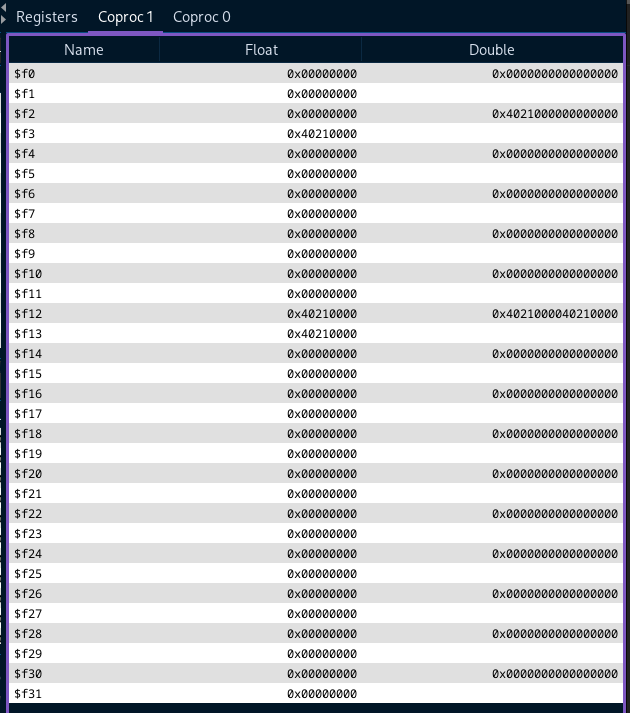
\includegraphics[width=0.6\textwidth]{image.png}
  \end{figure}
  
  En MIPS, los números de punto flotante de doble precisión (double) ocupan dos registros consecutivos de punto flotante. Como se puede ver en la imagen, al guardar el double num1 en \$f2, también MIPS lo guarda en \$f3 pero en tipo float.
  
  \begin{itemize}
  \item \textbf{Registro Par (Inferior):}
    El registro par (en este caso \$f2) contiene la mitad inferior de los 64 bits del double, 0x4021000000000000. Lo mismo para el registro \$f12 en un principio.
    
  \item \textbf{Registro Impar (Superior):}
    El registro impar siguiente (en este caso \$f3) contiene la mitad superior de los 64 bits del double, 0x40210000 Lo mismo se guarda en el resigtro \$f13.
  \end{itemize}
  
  Después en la línea \texttt{add.s \$f12 \$f3 \$f0} cargamos desde memoria, la mitad inferior 0x40210000 y la mitad superior 0x40210000. Es por eso que tenemos al final 0x4021000040210000 está almacenado en \$f12.
  
  Cómo última mencion, al correr el programa, la primer impresión del número es 8.5, que corresponde al primer valor guardado en \$f12 (0x4021000000000000) antes de la suma con el valor de la mitad inferior. Debajo se imprime 2.515625, que es el valor final asignado (0x4021000040210000) de la suma de la mitad inferior con la mitad superior.
  \bigskip

  \newpage
  
\item En MARS, en la barra de herramientas, en la pestaña de Tools, existe la herramienta llamada MIPS X-Ray, conecta esta herramienta y corre un programa línea por línea. ¿Qué significan los números resaltados de color magenta, verde, azul y azul claro que se encuentran abajo de la instrucción?
  \bigskip
  % -- Respuesta -- %

  \begin{figure}[H]
    \centering
    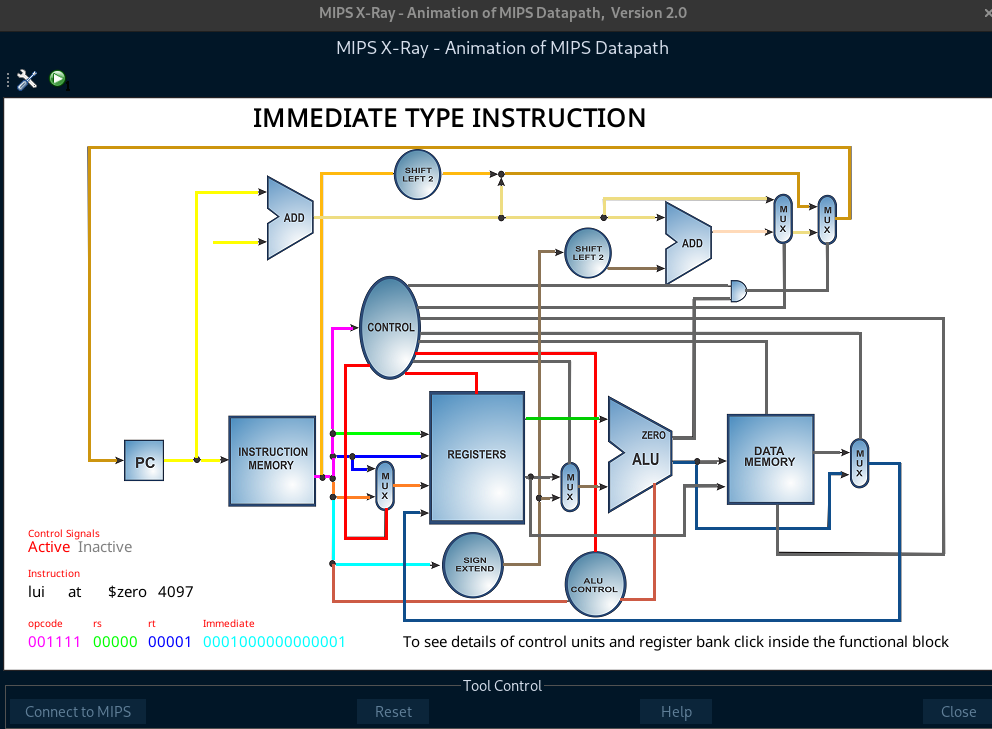
\includegraphics[width=0.9\textwidth]{image1.png}
  \end{figure}

  Los números resaltados en colores son los diferentes campos de la instrucción MIPS en formato de código de máquina.

  \begin{itemize}
  \item \textcolor{magenta}{\textbf{Magenta (001111):}} Como se ve en la imagen es el \textit{opcode}, el cual indica el tipo de instrucción. 001111 corresponde a la instrucción lui \textit{(Load Upper Immediate)}.
    
  \item \textcolor{green}{\textbf{Verde (00000):}} Es el registro rs \textit{(source register)}. En la instrucción lui, este campo no se usa por lo que suele establecerse en 0.
    
  \item \textcolor{blue}{\textbf{Azul (00001):}} Es el registro rt \textit{(target register)}, donde se almacenará el valor inmediato cargado en la parte alta del registro. El cual corresponde al registro \$at.

  \item \textcolor{cyan}{\textbf{Azul claro (0001000000000001):}} Representa el valor inmediato \textit{(Immediate)}. En el lui, este valor se coloca en los 16 bits superiores del registro destino. El inmediato salió como 4097 en decimal.
    
  \end{itemize}
  \bigskip
  
\end{enumerate}
\end{document}
